\subsection{Teléfono Inteligente}

\par
El teléfono inteligente (smartphone en inglés) es un tipo de computador de bolsillo que combina los elementos de una computadora con los de un teléfono celular; sobre una plataforma informática móvil, con mayor capacidad de almacenar datos y realizar actividades y con una mayor conectividad que un teléfono móvil convencional. El término inteligente, que se utiliza con fines comerciales, hace referencia a la capacidad de usarse como un computador de bolsillo, y llega incluso a reemplazar a una computadora personal en algunos casos\cite{smartphone}.

\par \noindent
Entre otros características comunes de los teléfonos inteligentes están:\cite{smartphone}

\begin{itemize}
\item La función multitarea;

\item El acceso a Internet vía Wifi o redes 2G, 3G o 4G;

\item La función multimedia (cámara y reproductor de videos/mp3);

\item Los programas de agenda y administración de contactos;

\item Acelerómetros, GPS y algunos programas de navegación;

\item La función de leer documentos de negocios en variedad de formatos como PDF y Microsoft Office
\end{itemize}

\par \noindent
Los sistemas operativos móviles más frecuentes utilizados por los teléfonos inteligentes, como se pueden observar en la figura 1.1, son:\cite{smartphone}

\begin{itemize}
\item Android, desarrollado por Google;

\item iOS, desarrollado por Apple;

\item Windows 10, desarrolla por Microsoft
\end{itemize}

\begin{figure}[H]
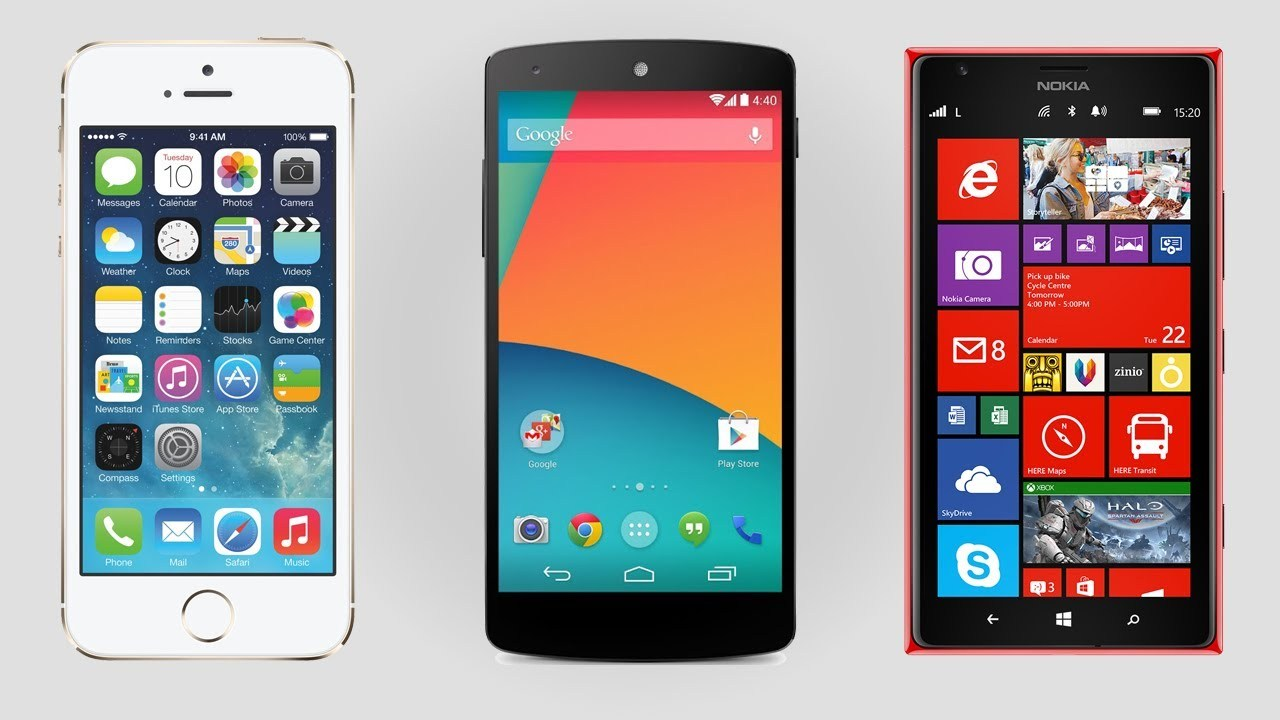
\includegraphics[width=\textwidth]{smartphone1.jpg}
\caption{Smartphones con los Sistemas Operativos iOS, Android y Windows Phone, respectivamente}
\end{figure}

\par \noindent
En el trabajo se desarrolló para el prototipo, una aplicación en el sistema operativo móvil Android, debido a su popularidad en el mercado y su vasta documentación para desarrollar aplicaciones.

